%_________________________________________________________________
%|                                  ihmtc.tex                    |
%| Template for IHMTC-2017 articles using LaTeX                  |
%| Created by   Dr. Supradeepan K                                |
%|              Department of Mechanical Engineering             |
%|              BITS-Pilani, Hyderabad Campus,                   |
%|              Hyderabad, India - 500 078.                      |
%|              Tel: (91) 40- (office)                           |
%|              Email: supradeepan@hyderabad.bits-pilani.ac.in   |                            
%|              WWW:                                             |
%|              May, 2017                                        |
%________________________________________________________________|


\documentclass[twocolumn,10pt,cleanfoot]{ihmtc}
\usepackage[T1]{fontenc}
\usepackage{balance}
\usepackage{amsmath}
\usepackage{amsfonts}
\usepackage{amssymb}
\usepackage{bm}

%

\usepackage{caption}
\usepackage{subcaption}
\captionsetup[subfigure]{justification=justified,singlelinecheck=false}
\usepackage{graphicx}
\graphicspath{{images/}}
\setlength{\belowdisplayskip}{5pt}
\setlength{\abovedisplayskip}{5pt}

\special{papersize=8.5in,11in}
\conffullname{the 24th National and 2nd International ISHMT-ASTFE\\
		Heat and Mass Transfer Conference (IHMTC-2017),}

%%%%% for date in a single month, use
%\confdate{24-28}
%\confmonth{September}
%%%%% for date across two months, use
\confdate{December 27-30}
\confyear{2017}
\confcity{BITS-Pilani, Hyderabad}
\confcountry{India}

%%% Use the number supplied to you 
%%% by Conference Secretariat for your paper
\papernum{IHMTC2017-06-0285}

%%% You need to remove 'DRAFT: ' in the title for the final submitted version.
%\title{\textsc{Paper Title}}
\title{Designed Periodic Cellular Materials for Enhanced Air-cooled Heat Sinks}
%%% first author
\author{Saksham Gakhar
\affiliation{Indian Institute of Technology Bombay\\saksham.gakhar94@gmail.com}
   
    }	

    

%%% second author
%%% remove the following entry for single author papers
%%% add more entries for additional authors
\author{Shankar Krishnan\thanks{Corresponding Author}
\affiliation{Professor, Indian Institute of Technology Bombay\\kshankar@iitb.ac.in}
   
    }	



\begin{document}

\maketitle 

\begin{abstract}
{\it \small
Stochastic metal foams available commercially enable multifunctional applications. However, stochastic metal foams with cells of random shape, morphology and distribution, often place materials in locations where their contribution to overall material properties is near negligible. The major drawback is the lack of control of open-cell mesostructures. On the other hand, periodic cellular structures lend themselves well to topology optimization \& integration of multiple functions enabling superior performance benefits. We present a `designed' periodic structured heat sink approach for enhancement of air-cooling of a heated substrate. Open-cellular periodic structures in a corrugated arrangement (similar to pleated filters or wall-flow filters) are mounted on the substrate as fin materials for high-performing heat sinks for applications in electronics cooling as they are likely outperform existing heat sink designs. Corrugated structures for these porous foam fins offer high effective surface area and lend themselves well to heat transfer density maximization subject to topological constraint that ensures highly uniform flow distribution of incoming flow across the serpentine geometry. To design periodic structures, a two-pronged approach is undertaken. The analytical investigation deals with an approximate yet reliable model for the flow distribution in the corrugated system as well as a means of theoretically approximating optimal geometrical topology (porosity) that leads to maximal heat transfer density at the microscopic level. The computational prong of the investigation helps corroborate results from the analytical model and in making the suitable decisions leading to the choice of the optimal geometry for macroscopic heat transfer density optimisation with special emphasis on the study of uniformity of flow through the system. The parametric study through numerical computations and the analytical model together help integrate the macroscopic and microscopic heat transfer optimisation schemes.
}
\end{abstract}


\begin{nomenclature}
%---> Modify between these comments
\entry{}{\textbf{Symbols} (S.I.)}
\entry{$A$}{area of cross section}
\entry{$V,U$}{velocities}
\entry{$v,u$}{non-dimensional velocities}
\entry{$u_{mean-j}$}{mean pore velocity for case $ j $}
\entry{$d$}{diameter of pore}
\entry{$P$}{static pressure}
\entry{$\Delta P$}{Pressure head}
\entry{$n$}{number of (cylindrical) pores}
\entry{$L_C$}{length of conduit (laterally)}
\entry{$L_p$}{pore length}
\entry{$ A_s $}{cross-sectional area of porous screen}
\entry{$w$}{width of the conduit}
\entry{$s$}{flow distribution metric}
\entry{$C_{fi}$}{coefficient of loss due to fluid's turning from intake conduit into the pore}
\entry{$C_{fe}$}{coefficient of loss due to fluid's turning from the pore into the exhaust conduit}
\entry{$f_c$}{average skin friction coefficient in the cylindrical pore}
\entry{$Re$}{Reynolds number}
\entry{$ T $}{Temperature}
\entry{$q$}{heat transfer rate ($W$)}
\entry{$q'''$}{heat transfer rate per unit volume ($W/m^3)$}
\entry{$R_{thermal}$}{= $\Delta T / q'''$, thermal resistance}
\entry{$k$}{thermal conductivity}
\entry{$C_p$}{specific heat capacity}
\entry{$x,y$}{cartesian coordinates}
%%
\entry{}{\textbf{Greek symbols}}
\entry{$\beta$}{$=V/V_c$, ratio of the upstream velocity of fluid in the inlet conduit to the axial component of velocity of the fluid that branches off into (in case of $\beta_i$) or joins from (in case of $\beta_e$) the pore}
\entry{$\rho$}{mass density}
\entry{$\mu$}{dynamic viscosity}
\entry{$\tau$}{shear stress}
%%
\entry{}{\textbf{Subscripts}}
\entry{$i$}{for quantities in the inlet conduit}
\entry{$e$}{for quantities in the exit (or exhaust) conduit}
\entry{$c$}{lateral channel (or pore, cylinder)}
\entry{$w$}{wall}
\entry{$p$}{pore}
\entry{$ \infty $}{incoming ambient stream}
%---> Modify between these comments
\end{nomenclature}

%\section{INTRODUCTION}
%
%%%%%%%%%%%%%%%%%%%%%%%%%%%%%%%%%%%%%%%%%%%%%5
\section{HEAT SINK TOPOLOGY}
%
We are considering the design of a heat sink where the aim is to cool a heated base plate by blowing a fluid over it. The process can be made efficient by deployment of fins which are
available in a variety of configurations, the most popular ones being
the parallel plate and pin-shaped fins. Prospective `designed' periodic cellular materials like porous metal
foams not only offer the advantage of being light in weight but also offer high effective surface
area (for a given volume with respect popular alternative heat fins). They have also proved to be good acoustic absorbers \cite{BM_U}. From a heat transfer
perspective, the large effective surface area is clearly a plus. Another extremely important requirement for many applications especially in heat sinks for electronics cooling, besides good heat transfer capability, is a lower pressure drop across the system. To this
end, we propose the use of a serpentine corrugated geometry of periodic
cellular material as the fin structure. Periodic cellular materials, unlike stochastic metal foams, offer great ease from the manufacturing perspective as well as a handsome control over the system's effective thermo-physical properties. Filling the entire heated
surface with metal foams looks like an attractive option from a heat
transfer vantage point but such a configuration is bound to offer
unreasonably high pressure drops for the cooling fluid medium, and thus does not quite qualify for an efficient
heat sink. Past research \cite{gallego2003carbon} has shown that although parallel plate fin configuration
offers extremely low pressure drops, the heat transfer rate could still
be improved by the use of pin-fins but at the cost of a higher pressure
drop. The idea behind the design discussed here is to exploit the higher heat transfer capability of
periodic cellular porous materials and the low pressure drops offered
by the corrugated geometry \cite{aboelsoud2013study} such that the trade-off between improved
heat transfer and lowered pressure drop typically encountered in other
popular alternatives is necessarily overcome.
%
\subsection{Periodic Unit Cell}\label{periodicunitcell}
The lower picture in Fig. (\ref{exploded}) shows a heat sink with periodic cellular foam as fins that are mounted in serpentine corrugations over a heated substrate. Considering applications in the electronics industry, the cooling medium is typically air. The figure also shows the exploded view of the self-repeating unit cell under consideration. A detailed sketch of the same unit cell is given in Fig. (\ref{simunitcell}).
%
\begin{figure}[ht]
\centerline{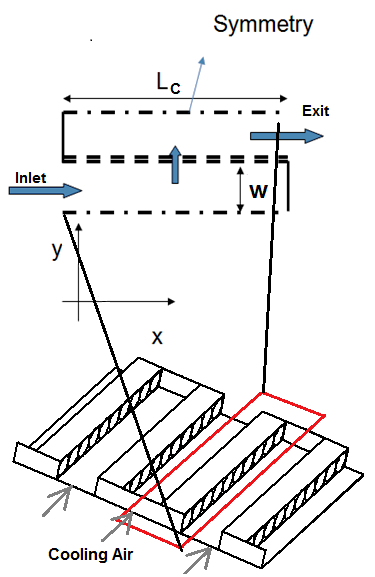
\includegraphics[width=80mm,height=120mm]{exploded_2.png}}
\vspace{-1.5ex}
\caption{\small{THE LOWER PICTURE DEPICTS THE HEAT SINK WITH PERIODIC CELLULAR MATERIAL ARRANGED IN CORRUGATIONS. THE ABOVE PICTURE SHOWS THE EXPLODED VIEW OF A UNIT CELL}}
\label{exploded}
\end{figure}
%
An important approximation made at this juncture for the periodic porous fin structure is that it is composed of laterally stacked pores all with tortuosity equal to unity, thereby simplifying the pores to laterally stacked cylinders. In practice, it is understood that this cellular structure is 3-D and has a corresponding permeability matrix, but we make another approximation by modelling this porous screen by only a single layer of cylinders that act as channels between the inlet conduit and the exit conduit. As a consequence, there is no permeability for flow between the cylinders or in other words, flow is restricted to take a 90$^\circ$ bend when it enters or leaves this cylindrical channel and thereby to flow axially through these cylindrical pores (thus a 1-D flow through the pores).
%
\begin{figure}[ht]
\centerline{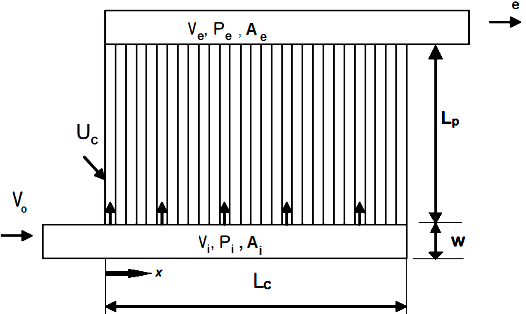
\includegraphics[width=80mm,scale=0.50]{unitcell.PNG}}
\vspace{-1.5ex}
\caption{\small{UNIT CELL OF THE CORRUGATED PERIODIC CELLULAR MATERIAL DEPLOYED AS FIN FOR THE HEAT SINK}}
\vspace{-2.2em}
\label{unitcell}
\end{figure}
%
%%%%%%%%%%%%%%
\section{ANALYTICAL MODELLING}
\subsection{Flow Distribution}\label{BMmodel}
In order to develop a theoretical understanding for the flow distribution
across the modelled unit-cell and the pressure drop across it, the most
basic mass and momentum balance principles have been invoked on flow
elements in that intake and exit conduits. The resultant mathematical
model that describes the flow behaviour reveals an important non-dimensional
parameter ($m^2$) which broadly captures the effect of important
design parameters and whose relative magnitude (with respect to similar
alternate design configurations) necessarily reveals the degree of
the flow uniformity. The model also provides insight on the scaling
of the pressure drop across the heat sink unit cell given a particular
value of $m^2$. \\
%
%%
%
All calculations for the model are based on one-dimensional flow equations
under simplifying assumptions. As discussed in section \ref{periodicunitcell}, the panel of lateral pores is modelled
as a single layer of adjacently stacked thin cylinders of diameter
$d$ and length $L_p$. These are assumed to have a wall thickness
$<<$ any of the characteristic dimensions. These lateral
pores form right-angled junctions to either of the conduit
axes. In the dividing-flow-type inlet conduit, the fluid progresses
and as it approaches the lateral pore, some fluid is lost through
it and the remainder of the flow proceeds downstream at an ever decreasing
flow rate. In the combining flow case in the exit conduit, fluid approaches
the branch point along both the conduit and the lateral pore (cylinder).
These fluid streams combine at the branch point and proceed downstream along the conduit at an ever increasing flow rate. Primary
frictional losses are accounted for by $90^{\circ}$ turning losses,
pore wall friction losses and expansion-contraction losses (when the fluid enters into and exits from the pores respectively). \\
%
%%
%
Consider an incompressible fluid flowing isothermally along the inlet
conduit of uniform cross- sectional area $A_i$ as illustrated in
Fig. (\ref{unitcell}). The control volume at the mouth of a pore is shown with dotted line in Fig. (\ref{inletcon}). A part of
the incoming flow branches into the lateral pore as a result of the
pressure difference in the inlet conduit and the ambient. $P_i(x)$
is the static pressure at a location $x$ in the inlet conduit. Since
the flow decelerates due to loss of fluid to the lateral pore, the
pressure $P_i(x+\Delta x)$ is greater than the upstream pressure
$P_i(x)$. Fluid is transported to the lateral pore with a normal
velocity $U_c$ while retaining an axial velocity component $V_c$. 
%
\begin{figure}[ht]
\centerline{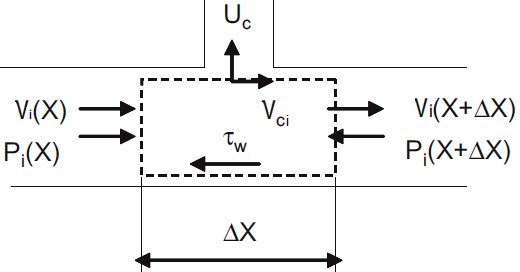
\includegraphics[width=80mm,scale=0.50]{inletcon.PNG}}
\vspace{-1.5ex}
\caption{\small{A FLUID CONTROL VOLUME IN THE INLET CONDUIT. A FRACTION OF FLUID BRANCHES INTO THE PORE}}
\label{inletcon}
\vspace{-3em}
\end{figure}
%
Using the principle of mass balance, we thus
have%
\begin{equation} \label{in-mass}
\rho {{A}_{i}}{{V}_{i}}=\rho {{A}_{i}}({{V}_{i}}+\frac{d{{V}_{i}}}{dx}.\Delta x)+\rho {{A}_{c}}{{U}_{c}}
\end{equation}
%
Solving for normal velocity of fluid inside the pore, one gets
%
\begin{equation} \label{in-uc}
{{U}_{c}}\,=-\frac{{{A}_{i}}L_C}{{{A}_{c}}n}.\frac{d{{V}_{i}}}{dx} 
\end{equation}
%
The principle of momentum balance for the axial $x$ direction on the control volume yields
%
\begin{equation} \label{in-mom}
\begin{split}
{{P}_{i}}A_i+\rho {{A}_{i}}{{V}_{i}}^{2}={A}_{i}({{P}_{i}}+\frac{d{{P}_{i}}}{dx}\Delta x) & +{\tau }_{w}\pi {d}_{i}\Delta x \\
& +\rho {A}_{i}{({{V}_{i}}+\frac{d{{V}_{i}}}{dx}\Delta x)}^{2}+\rho {{A}_{c}}{{U}_{c}}{{V}_{c}}
\end{split}
\end{equation}
%
Now assuming the Darcy-Weisbach correlation ${{\tau }_{w}}=f_c\frac{\rho {{V}_{i}}^{2}}{8}$
to hold true in the conduit, and upon neglecting higher order terms
of $\Delta x$, we have :
%
\begin{equation} \label{in-mom-final}
\frac{1}{\rho }.\frac{d{{P}_{i}}}{dx}+\frac{{{f}_{i}}}{2{{d}_{i}}}{{V}_{i}}^{2}+(2-{{\beta }_{i}}){{V}_{i}}\frac{d{{V}_{i}}}{dx}=0
\end{equation} where $\beta_i=\frac{V_i}{V_c}$ . 
%
\begin{figure}[ht]
\centerline{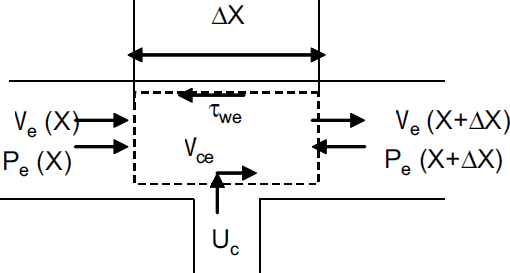
\includegraphics[width=80mm,scale=0.50]{exitcon.PNG}}
\vspace{-1.5ex}
\caption{\small{A FLUID CONTROL VOLUME IN THE EXIT CONDUIT. A FRACTION OF INCOMING FLUID FROM THE PORE JOINS THE MAIN PASSAGE FLOW}}
\label{exitcon}
\end{figure}
%
Similar to the inlet conduit mass balance eqs. (\ref{in-mass},\ref{in-uc}), the mass balance on control volume shown in Fig. (\ref{exitcon}) on the exit conduit gives
%
\begin{equation} \label{out-uc}
{{U}_{c}}\,=\frac{{{A}_{e}}L_C}{{{A}_{c}}n}.\frac{d{{V}_{e}}}{dx}
\end{equation}
%
Similar to eq. (\ref{in-mom-final}), the momentum balance principle on the control volume shown in Fig. (\ref{exitcon}) on the exit conduit yields
%
\begin{equation} \label{out-mom-final}
\frac{1}{\rho }\frac{d{{P}_{e}}}{dx}+\frac{{{f}_{e}}}{2{{d}_{e}}}{{V}_{e}}^{2}+(2-{{\beta }_{e}}){{V}_{e}}\frac{d{{V}_{e}}}{dx}=0
\end{equation}
%
Eqs. (\ref{in-uc}) and (\ref{out-uc}) together yield the following
relation between the inlet and the exit conduit velocities at any
$x$ under the boundary condition $V_e=0$ at $x=0$ and $V_i=V_o$ at $x=0$ :
%
\begin{equation} \label{vel-relation}
{{V}_{e}}=\left( {{V}_{o}}-{{V}_{i}} \right)\frac{{{A}_{i}}}{{{A}_{e}}}
\end{equation}
%
Now subtracting eq. (\ref{out-mom-final}) from eq. (\ref{in-mom-final}),
we get the following : 
%
\begin{equation} \label{combined-mom}
\begin{split}
\frac{1}{\rho}\frac{d({{P}_{i}}-{{P}_{e}})}{dx}+\frac{{f}_{i}}{2{{d}_{i}}}{{V}_{i}}^{2}-\frac{{f}_{e}}{2{{d}_{e}}} & {{V}_{e}}^{2} +(2-{\beta}_{i}){V}_{i}\frac{d{{V}_{i}}}{dx}\\ 
& - (2-{\beta }_{e}){V}_{e}\frac{d{{V}_{e}}}{dx}=0
\end{split}
\end{equation}
%
Additionally, we write the pressure drop across a pore at a location
$x$ as follows : 
%
\begin{equation} \label{zeta-def}
{{P}_{i}}-{{P}_{e}}=\rho(1+{{C}_{fi}}+{{C}_{fe}}+{{f}_{c}}\frac{{{l}_{c}}}{{{d}_{c}}}){{U}_{c}}^{2}=\rho \zeta \frac{{{U}_{c}}^{2}}{2}
\end{equation}where $C_{fi}$ is coefficient of turning loss encountered when the fluid in the control volume bends from the intake conduit
into the lateral pore and $C_{fe}$ is the coefficient of turning loss encountered when the fluid bends from the
lateral pore into the exhaust conduit, and $f_c$ is average skin friction coefficient for the flow through the pore.
%
Now using relations in eqs. (\ref{in-uc},\ref{out-uc},\ref{vel-relation},\ref{zeta-def})
to simplify eq. (\ref{combined-mom}) above and also non-dimensionalising the resultant simplified equation with ${{p}_{i}}=\frac{{{P}_{i}}}{\rho{{V}_{o}}^{2}},{{p}_{e}}=\frac{{{P}_{e}}}{\rho{{V}_{o}}^{2}}{{v}_{i}}=\frac{{{V}_{i}}}{{{V}_{o}}},{{v}_{e}}=\frac{{{V}_{e}}}{{{V}_{o}}},{{u}_{c}}=\frac{{{U}_{c}}}{{{V}_{o}}},X=\frac{x}{L}$,
we get the following control equation that governs the velocity variation : 
%
\begin{equation} \label{controleq}
\frac{{{d}^{2}}(1-{{v}_{i}})}{d{{X}^{2}}}-{{m}^{2}}(1-{{v}_{i}})=\varepsilon
\end{equation}%
%
where 
%
\begin{equation} \label{msq}
\varepsilon\,=\frac{\left( 2-{{\beta }_{i}} \right)}{\zeta{{\left[\frac{{{A}_{i}}}{n{{A}_{c}}} \right]}^{2}}}\,\,\,\,\text{   and    }\,\,\,\,{{m}^{2}}=\left\{ \left[ \frac{2-{{\beta }_{e}}}{2-{{\beta }_{i}}} \right].{{\left[ \frac{{{A}_{i}}}{{{A}_{e}}} \right]}^{2}}-1 \right\}.\varepsilon
\end{equation}
%
%
This control equation can be solved under the known boundary conditions
$v_i=1$ at $x=0$ and $v_i=0$ at $x=1$. The solution will be different
depending on the sign of $m^2$. Evaluating the value and sign of this parameter in turn requires the knowledge of the parameters $\beta_i$, $ \beta_e $ and $\zeta$. It has been found from a large set
of computational data that for all practical purposes $\beta_i \simeq 0.8$
and $0.02 \leq \beta_e \leq 0.1$. As for the value of $\zeta$, it differs from configuration to configuration and depends on the ratio of the channel to conduit cross sectional areas and ratio of the corresponding flow rates. The value of $\zeta$ can be calculated from its equivalent representation as in terms of the loss coefficients presented in eq. (\ref{zeta-def}). We can therefore express $f_c$, the Darcy friction factor as $64/Re$ from the knowledge that the flow through the cylindrical channel is essentially laminar. The loss  coefficients are constituted of the contraction and inlet turning losses for $C_{fi}$ and expansion and exit turning losses for $C_{fe}$. The values of $C_{fi}$ and $C_{fe}$ for each system are calculated from the correlations observed in ref. \cite[Chapter~7]{idelchik2005handbook}. The sign of $m^2$ is dictated by the relative magnitudes of $\beta$'s and for our case, it is necessarily $>0$. Although eq. (\ref{controleq}) has been solved for cases where $m^2\leq0$, here we only present the solution for cases where $m^2>0$.\\
%%%%%%%%%%%%%%%%%m_sq>0 solution%%%%%%%%%%%%%%%%%%%%%%%%%%
\textbf{Inlet Conduit velocity ($\bm{v_i}$)}
\begin{equation}\label{vi} 	
\begin{split}
{v}_{i}=1-\left( \frac{\sinh (mX)}{\sinh (m)} \right)+\frac{\varepsilon }{{m}^{2}}\Biggl[ 1 & - \left( \frac{\sinh (mX)}{\sinh (m)} \right) \\
& -\left( \frac{\sinh (m(1-X))}{\sinh (m)} \right) \Biggr]
\end{split}
\end{equation}
%
%
\textbf{Exit Conduit velocity ($\bm{v_e}$)}
\begin{equation}\label{ve}
{v}_{e}=\left( 1-{v}_{i} \right)\frac{{A}_{i}}{{A}_{e}}
\end{equation}
%
%
\textbf{Channel Velocity ($\bm{u_c}$)}
\begin{equation} \label{uc} 
\begin{split}
{u}_{c}=\left(\frac{{A}_{i}}{{{A}_{c}}n} \right) & \left( \frac{m}{\sinh (m)} \right) \Biggl[ \cosh (mX)  \\ 
 & + \frac{\varepsilon }{{m}^{2}}\biggl( \cosh (mX)-\cosh (m(1-X)) \biggr) \Biggr]
\end{split}
\end{equation}
%
%
\textbf{Local pressure drop ($\bm{p_i-p_e}$)}
\begin{equation} \label{dp} 
\begin{split}
{p}_{i}-{p}_{e}=\frac{\zeta}{2} & \left( \frac{{A}_{i}}{{{A}_{c}}n} \right)^{-2}\; {\biggl( \frac{m}{\sinh (m)} \biggr)}^{2}\Biggl\{ \cosh (mX)\\
& +\frac{\varepsilon }{{m}^{2}}\biggl( \cosh (mX) - \cosh (m(1-X)) \biggr) \Biggr\}^{2}
\end{split}
\end{equation}
%
%
\textbf{Net pressure drop ($\bm{\Delta P}$)}
\begin{equation} \label{netdp} 
\begin{split}
\Delta P=\biggl({{\left. {{p}_{i}} \right|}_{X=0}}-{{\left. {{p}_{e}} \right|}_{X=1}}&\biggr)=\frac{\zeta}{2} {\left( \frac{{A}_{i}}{{{A}_{c}}n} \right)}^{-2}\; \Biggl\{{{\left( \frac{m}{\tanh (m)} \right)}^{2}} \\
& +\varepsilon \left( 1+\frac{\varepsilon }{{{m}^{2}}} \right){{\left( \frac{\left( 1-\operatorname{sech}(m \right)}{\tanh (m)} \right)}^{2}} \Biggr\}  
\end{split}
\end{equation} 
%
%
\subsection{Existence of Optimal Geometry}\label{existence_dopt}
The choice of length scales for heat transfer devices including but not limited to heat sinks pose the fundamental problem of demarcation of permissible optimal ranges of these lengths from a design perspective; the aim of which is to maximise heat transfer density through the device within a fixed volume. In our case, considering the flow through laterally stacked cylinder as shown in Fig. \ref{simunitcell}, an essential component of the design cycle is the choice of  optimal flow channel size and optimal porosity of the assembly.
%
\begin{figure}[ht]
\centerline{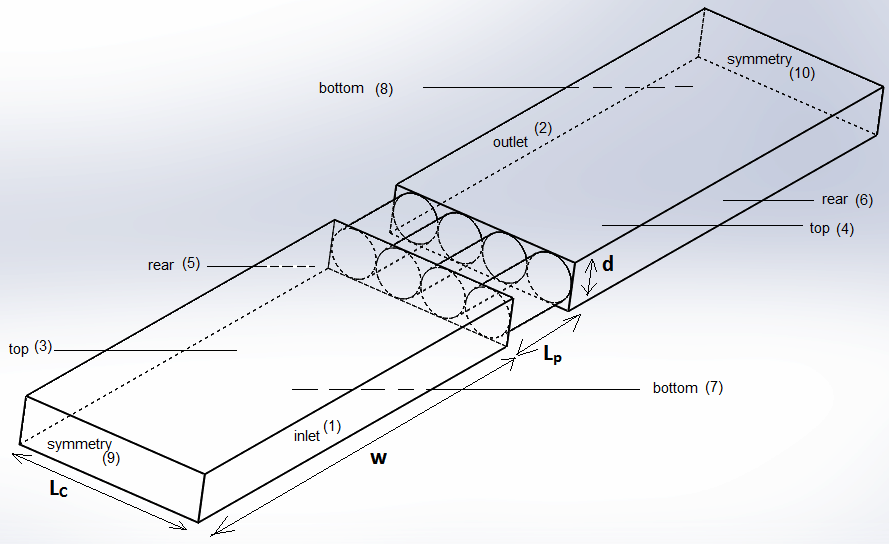
\includegraphics[height=0.65\linewidth,width=1\linewidth]{simunitcell.png}}
\vspace{-1ex}
\caption{\small{SOLIDWORKS MODEL OF THE UNIT CELL}}
\vspace{-1.5em}
\label{simunitcell}
\end{figure}
%
The problem becomes an unconventional one because with the increasing miniaturisation of scales, the regimes of operation tend to those where the slenderness assumption starts to break ($d/L_C$ not $<< 1$) along with which common heat transfer premises such as boundary layer theories and correlations become invalid and misleading. In this section, we address the question of existence of an optimal design range for channel (or equivalently the porosity) through analytical means. The question of the right choice of channel geometry will then be addressed in section \ref{choiceofdesign}. This latter decision will in part be governed by other macroscopic requirements for
overall heat transfer density like increased degree of flow uniformity.
%
\subsubsection*{Optimal geometry in the small-scale limit:} In the limit of decreasing length scales, consider the limit of dimensions $ d $ and $ L_C $ such that $d/L_C$ is not $<< 1$. There are three flow configurations under which heat sinks are typically used depending on how the heat sink is attached to the cooling network \cite{types_of_cooling_configs}. These are : first, a fixed pumping power; second, a fixed pressure drop; and third, a fixed mass flow rate. Here we consider the case where the pressure drop $ \Delta P $ across the heat sink and hence the periodic unit cell under study is fixed. The analysis presented next can nevertheless be extended to the other two configurations as well by appropriately changing the relation between the mean velocity and $\Delta P$.\\
%
In case $ (a) $, the first extreme, there are so many pores packed in the same volume such that the diameter $ d $ is so tight that owing to excellent wall-fluid thermal contact, the exiting flow through the pore can be assumed to be at the same temperature as the wall ($ T_w $). In other words, the flow can be seen to be approximately like a Hagen-Poiseuille \emph{`type'} fully developed channel flow. In this case $ (a) $ therefore, we can approximate the mean pore axial velocity to be 
%
\[u_{mean-a}=\frac{{d}^{2}}{32\mu }\frac{\Delta P}{{L}_{p}}\]
%
Since the cylinders have very thin walls (with thicknesses $\sim d/100 $) the total flow area for the porous screen, $ A_s $, is approximately equal to $n \times$ {\it cross sectional area of one pore}. Therefore, the total heat transfer is $ q=\dot{m}C_p(T_w-T_\infty) $, where $ T_\infty $ is the temperature of the incoming stream of cooling fluid. Here $\dot{m}=\rho A_s u_{mean-a}$. The heat transfer density then becomes $ q''' =q/V$ where $ V $ is the volume to which heat is rejected ($ =A_s \times L_p$). Thus,
%
\begin{equation}\label{d0}
q'''({W}/{{m}^{3}})=\frac{\rho {{C}_{p}}(T_w-T_\infty)\Delta P}{32\mu }\frac{{{d}^{2}}}{{{L}_{p}}^{2}}
\end{equation}
%
In the other extreme case $ (b) $ of $d/L_C$ is not $<< 1$, we have the diameters that are large enough with respect to pore lengths such that the channels are no longer slender. In this increasing $d/L_C$ scenario, the boundary layer slenderness assumption breaks and contribution of convection mode of heat transfer becomes negligible with respect to conduction. Let the thickness of fluid film which surrounds the wall inside the channel be $ \delta $ which can be approximated, through dimensional analysis as $ 2\sqrt{\alpha t} $, where $t$ has the dimensions of time. It follows that,
\[\delta \simeq 2\sqrt{\alpha \frac{L_p}{u_{mean-b}}}\]
%
Furthermore, making the Bernoulli approximation we have,
\[u_{mean-b} \simeq \sqrt{\frac{2\Delta P}{\rho }}\]
%
Now, the conduction heat transfer from the wall to this fluid film can be written as $ q_1=k S (T_w-T_\infty)$, where $ S $ is the thermal shape factor for the film developed close to the wall. This is the heat transfer rate through one channel. Under the assumption of a near cylindrical film of thickness $\delta$ (with the inner radius of the annular cylinder being $d-\delta$ and outer being $d$), the expression becomes
\[q_1=k \left( \frac{2 \pi L_p}{ln\left(\frac{d}{d-\delta}\right)} \right) (T_w-T_\infty) \]
Now we can write : $ln(\frac{d}{d-\delta})=ln(1+\frac{\delta}{d-\delta}) \Rightarrow ln(1+\frac{\delta}{d-\delta}) \simeq \frac{\delta}{d-\delta}$. (This simplification uses the approximation : $ln(1+x) \simeq x$ if $x<<1$, where $x=\frac{\delta}{d-\delta}<<1$ in our case). Futhermore, we have $ln(\frac{d}{d-\delta})\simeq\frac{\delta}{d}$ because $d-\delta \simeq d$. The number of pores are $n=A_s/(\frac{\pi d^2}{4})$. Therefore total heat transfer rate through $n$ pores becomes
\[q=\biggl( \frac{4 A_s}{\pi d^2}\biggr) \frac{2 \pi k L_p d}{\delta}(T_w-T_\infty)\]
We are interested in the heat transfer density $q''' = q/V$, where again $V=A_s \times L_p$. Finally we get, 
%
\begin{equation}\label{dinf}
q'''(W/m^3)=\frac{4k (T_w-T_\infty)}{d}\left(\frac{2\Delta P}{\rho\alpha^{2}L_{p}^{2}}\right)^{1/4}
\end{equation}
%
Eqs. (\ref{d0}) and (\ref{dinf}) are the two asymptotes and these two clearly prove the existence of an optimal diameter of the pore for maximal heat transfer density (since eq. \ref{d0} has $q''' \propto d^2$ and eq. \ref{dinf} has $q''' \propto d^{-1}$). Therefore, by the method of matched asymptotes \cite{bejan2004declength}, $q'''$ is warranted to peak in the vicinity of the intersection of Eqs. (\ref{d0}) and (\ref{dinf}). Therefore the optimal spacing and maximal heat transfer density is given as 
%
\begin{equation}
\left(\frac{d}{L_{p}}\right)_{optimal} \simeq \frac{\left(128\mu\right)^{{1}/{3}}}{\left(\Delta P \, L_p^2 \right)^{{1}/{4}}}\left(\frac{2\alpha^{2}}{\rho}\right)^{{1}/{12}}
\end{equation}
%
\begin{equation}
q_{max}\,  \lessapprox \, \frac{k (T_w-T_\infty)}{L_p}\frac{\sqrt{\Delta P}}{(2\, \rho \mu^2 \alpha^4)^{1/6}}
\end{equation}
%%%%%%%%%%%%%%%%%%%%%%%%%%%%%%%%%%%%%%%%%%%%%%%
%%%%%%%%%%%%%%%%%%%%%%%%%%%%%%%%%%%%%%%%%%%%%%%
%%%%%%%%%%%%%%%%%%%%%%%%%%%%%%%%%%%%%%%%%%%%%%%
\section{COMPUTATIONAL MODELLING}\label{compmodel}
To examine the validity and accuracy of the solutions obtained using the above analytical models, the flow distribution and heat transfer is studied computationally where the self-repeating unit cell shown in Fig. (\ref{simunitcell}) has been chosen as the calculation domain for simulation in ANSYS Fluent commercial software. The most general system of governing equations for the single-component fluid which describe the mean flow properties, is cast in integral Cartesian form for an arbitrary control volume $V$ with differential surface area $d\boldsymbol{A}$ \cite{fluent} as follows
%
\begin{equation*}
\frac{\partial}{\partial t}\int_{V}\boldsymbol{W\:}dV+\iint_{A}\,[\mathbf{F}-\mathbf{G}].d\boldsymbol{A}=\int_{V}\boldsymbol{H\:}dV 
\end{equation*}
%
where the vectors $\boldsymbol{W}$, $\mathbf{F}$ and $\mathbf{G}$ are defined as 
%
\begin{equation*}
 \boldsymbol{W}=\left[\begin{array}{c} \rho\\ \rho u\\ \rho v\\ \rho w\\ \rho E \end{array}\right] ; \boldsymbol{\mathbf{F}}=\left[\begin{array}{c} \rho\boldsymbol{v}\\ \rho\boldsymbol{v}u+\rho\boldsymbol{i}\\ \rho\boldsymbol{v}v+\rho\boldsymbol{j}\\ \rho\boldsymbol{v}w+\rho\boldsymbol{k}\\ \rho\boldsymbol{v}E+p\boldsymbol{v} \end{array}\right] ; \mathbf{G}=\left[\begin{array}{c} 0\\ \tau_{xi}\\ \tau_{yi}\\ \tau_{zi}\\ \tau_{ij}v_{j}+\boldsymbol{q} \end{array}\right]
\end{equation*}
%
and $\boldsymbol{H}$ vector contains source terms such as gravity body-force and the heat generation terms. Here $\rho$, ${\mbox{\boldmath$v$}}$, $E$ and $p$ are the fluid density, velocity, total fluid energy per unit mass and pressure respectively. ${\mbox{\boldmath$\tau$}}$ is the viscous stress tensor, and ${\mbox{\boldmath$q$}}$ is the heat flux. \\
%
A second-order upwind flux scheme was used for the flow and the SIMPLE finite volume algorithm was used for obtaining the velocity fields. The calculations were terminated when the scaled residuals had dropped below ${{10}^{-7}}$ for all governing equations. The system is solved for steady state, incompressible, laminar and viscous flow of air ($\mu =1.81\times {{10}^{-5}}~$Pa.s and $\rho =1.225\,\text{kg/}{{\text{m}}^{3}}$). The thermo-physical properties have been assumed constant. 
%
The boundary conditions used in the simulations are enumerated next.
\begin{enumerate}     
\item {A velocity inlet boundary condition with a uniform value was assumed at the entrance of the inlet conduit (numbered 1 in Fig. \ref{simunitcell}). The inlet pressure was set to 50 Pa of gauge pressure. The inlet velocity magnitude for all the simulations is 1 m/s. The temperature of the incoming cooling fluid (air) has been assumed to be equal to the ambient (300 K).}
%         
\item{A nil gauge pressure outlet boundary condition was imposed on the outlet of the domain (numbered 2  in Fig. \ref{simunitcell}. The outlet is also assumed to be at ambient temperature.}
%         
\item{The top walls of both the inlet and exit conduits (numbered 3,4 in Fig. \ref{simunitcell}) and the rear walls of each conduit (numbered 5,6 in Fig. \ref{simunitcell}) are assumed to be stationary with the no-slip boundary condition. The constant temperature at these walls is assumed to be the same as ambient.}
%
\item{The bottom walls (numbered 7,8 in Fig. \ref{simunitcell}) and the walls of the laterally stacked cylinders are also assumed to be stationary with no-slip boundary condition. Here, unlike the top walls, a constant temperature thermal boundary condition has been imposed. These walls have been assumed ideal such that the thermal resistance in the can be ignored ($k_w \rightarrow \infty$). This implies that the bottom plate and the cylindrical fins can be assumed isothermal at 343 K.}
%       
\item{The two walls that lie along the length of the conduit (numbered 9,10 in Fig. \ref{simunitcell}) form the symmetry planes for the periodic unit cell. We impose the symmetry boundary condition on these walls which is equivalent to 0 shear stress along the wall hydrodynamically. This condition is invoked owing to the symmetry of the simulation geometry.}      
\end{enumerate}
%
%%%%%%%%%%%%%%%%%%%%%%%%%%%%%%%%%%%%%%%%%%%%%%%%%%%%%

\section{RESULTS AND DISCUSSION}
%
\subsection{Validation of the model}
Although it is feasible to reliably model and predict the fluid velocities and pressure drops in a prospective heat sink through numerical simulations, the path to such an analysis may not be the best when a suitable model, such as the one discussed in section \ref{BMmodel} can be used instead. In this section we present the comparison of local pressure drops across each of the cylindrical pores and inlet \& exit conduit velocity variations. The results have been obtained from the analytical model of section \ref{BMmodel} and from numerical simulations with specifics discussed in section \ref{compmodel}. The excellent corroboration between the numerical and analytical results makes it feasible to reliably predict the flow distribution through results of the analytical model. 
%
\subsubsection*{Inlet and exit conduit velocities:} It is not easy to numerically validate any given configuration since it is an expensive task both computation-wise and in time to generate unit cells for different configurations. However, it is relatively easier to validate the theoretical predictions for fluid velocities and pressure drops by varying the diameter $d$ and length of conduit $L_C$ (holding length of pore -- $L_p$, conduit width -- $w$ as constants) and studying the results for a variety of configurations. Figs. (\ref{velvalid_a}), (\ref{velvalid_b}) and (\ref{velvalid_c}) show the comparison of the $x$ variation of non-dimensional velocities for 3 different configurations. The dotted blue and black lines represent the analytical results for the $ x $ variation of the inlet and exit conduit velocities respectively. The computational results are in extremely good agreement not only for these 3 representative configurations, but also for other configurations tested over a wide range of $d/L_p$ and $L_C/w$ with maximum deviation between the two predictions being anywhere between 8-10$\%$.
%
\begin{figure}
\centering
   \begin{subfigure}[b]{0.55\textwidth}
   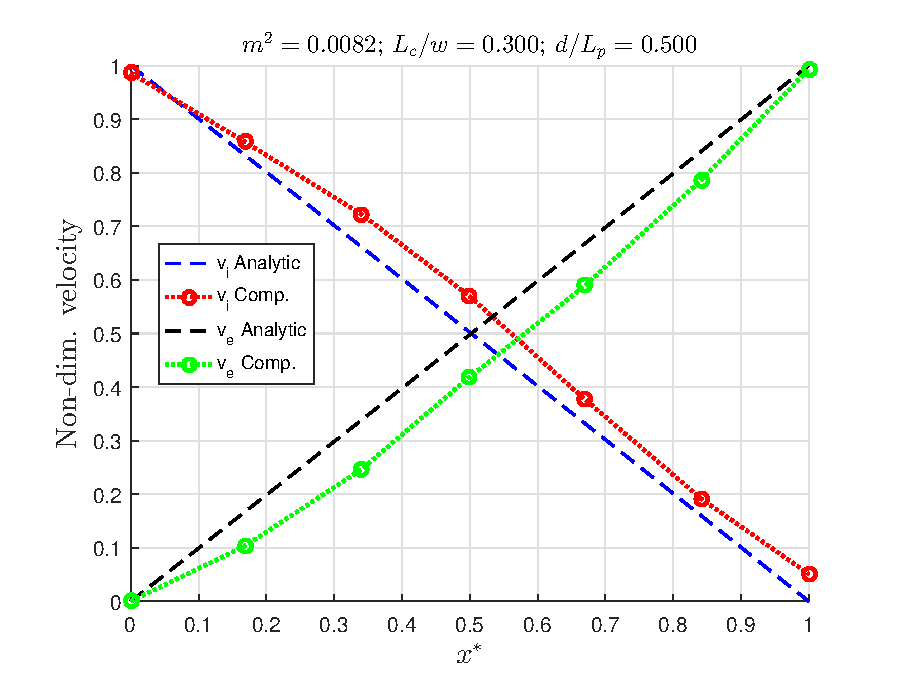
\includegraphics[height=0.55\linewidth,width=0.90\linewidth]{velvalid_a.eps}
    \caption{} 
   \label{velvalid_a} 
\end{subfigure}
%
   \begin{subfigure}[b]{0.55\textwidth}
   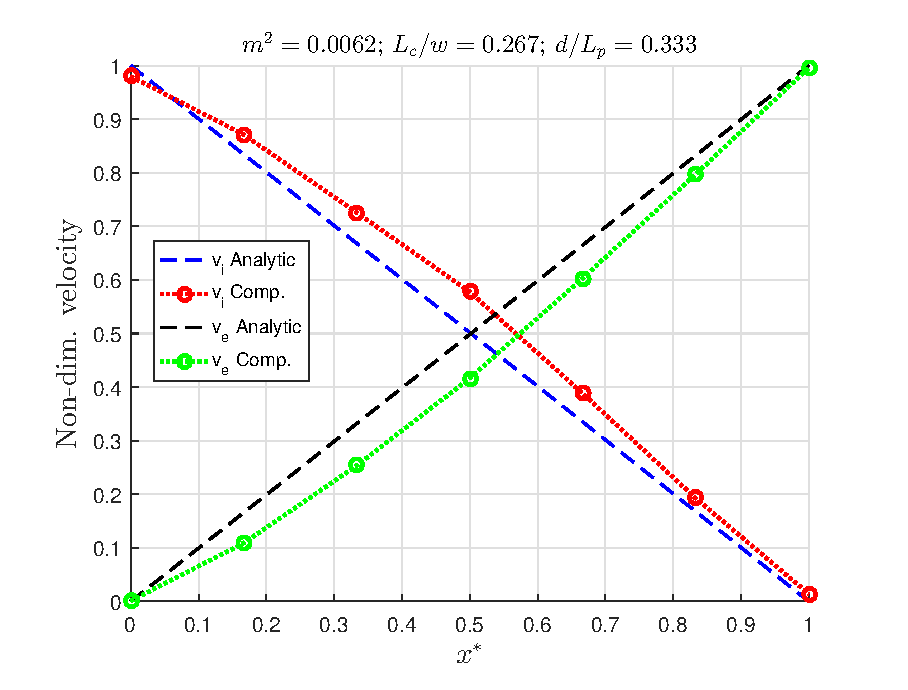
\includegraphics[height=0.55\linewidth,width=0.90\linewidth]{velvalid_b.eps}
   \caption{}
   \label{velvalid_b} 
\end{subfigure}
%
%
   \begin{subfigure}[b]{0.55\textwidth}
   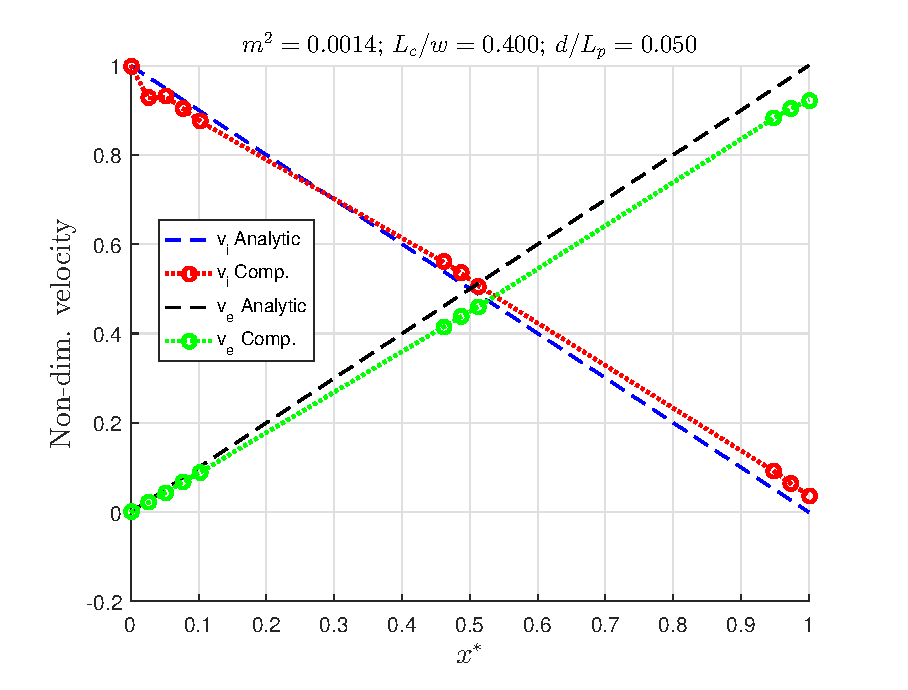
\includegraphics[height=0.55\linewidth,width=0.90\linewidth]{velvalid_c.eps}
   \caption{}
   \label{velvalid_c} 
\end{subfigure}
%
\caption{INLET \& EXIT CONDUIT VELOCITIES}
\vspace{-3em}
\end{figure}
%
%
\subsubsection*{Local pressure drops:} Here we present comparison of the local pressure drops through representative results as seen in Figs. (\ref{pres_a}), (\ref{pres_b}) and (\ref{pres_c}). It is important to remark here that the analytical model of section \ref{BMmodel} is based on a very important premise; it is that of completely uniform flow distribution in the conduits which in other words means nearly equal flow rate flowing through each of the porous channels. That is the reason why the model prediction of local pressure drops is nearly flat. In comparison to these, the numerical predictions show deviations because we are dealing with unoptimised cases here that don't yet represent perfect or near-perfect flow uniformity, which becomes the cause of some degree of deviation from the ideal results. This point will be elaborated and exploited in more detail in section \ref{choiceofdesign}. Nevertheless, the magnitudes are reasonably close and that makes the analytical model predictions a very good starting point for understanding flow distribution. 
%%%%
%
\begin{figure}
\centering
   \begin{subfigure}[b]{0.55\textwidth}
   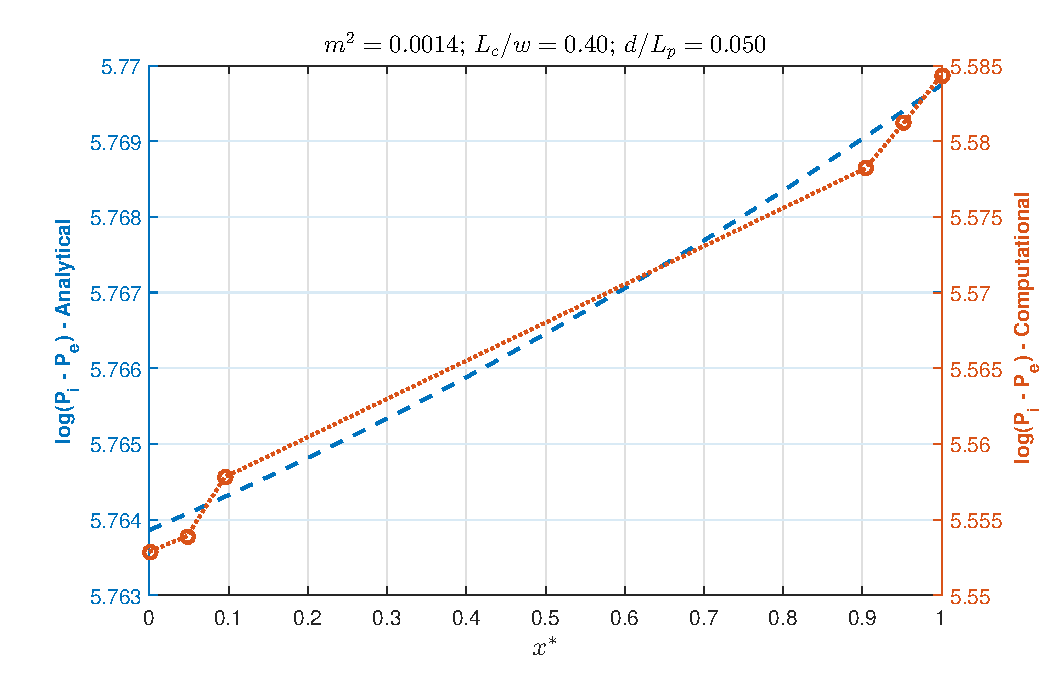
\includegraphics[height=0.55\linewidth,width=0.90\linewidth]{pres_a.eps}
   \caption{}
   \label{pres_a} 
\end{subfigure}
%
   \begin{subfigure}[b]{0.55\textwidth}
   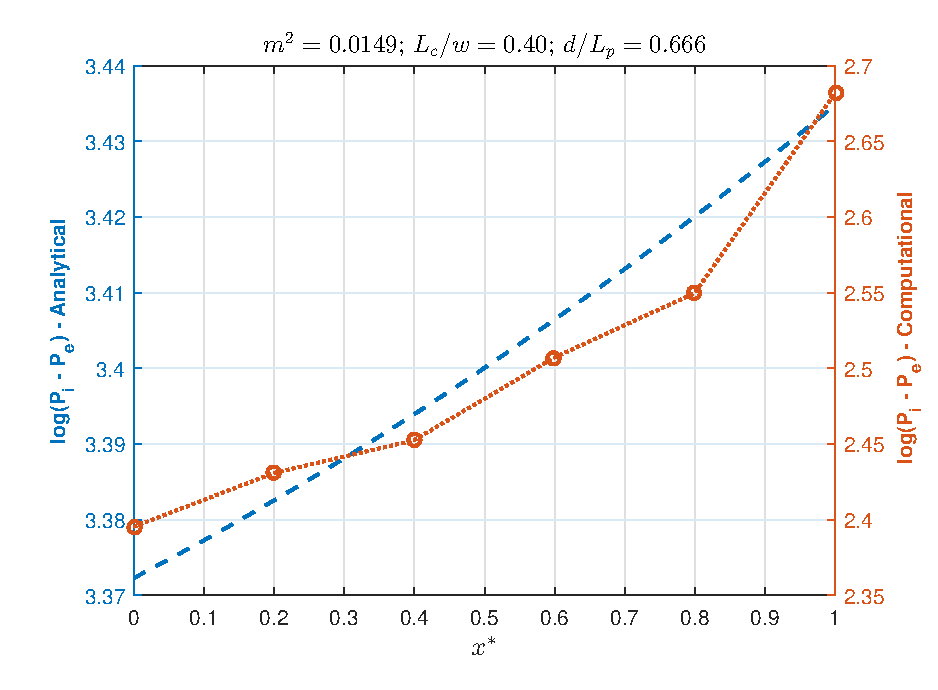
\includegraphics[height=0.55\linewidth,width=0.90\linewidth]{pres_b.eps}
   \caption{}
   \label{pres_b} 
\end{subfigure}
%
%
   \begin{subfigure}[b]{0.55\textwidth}
   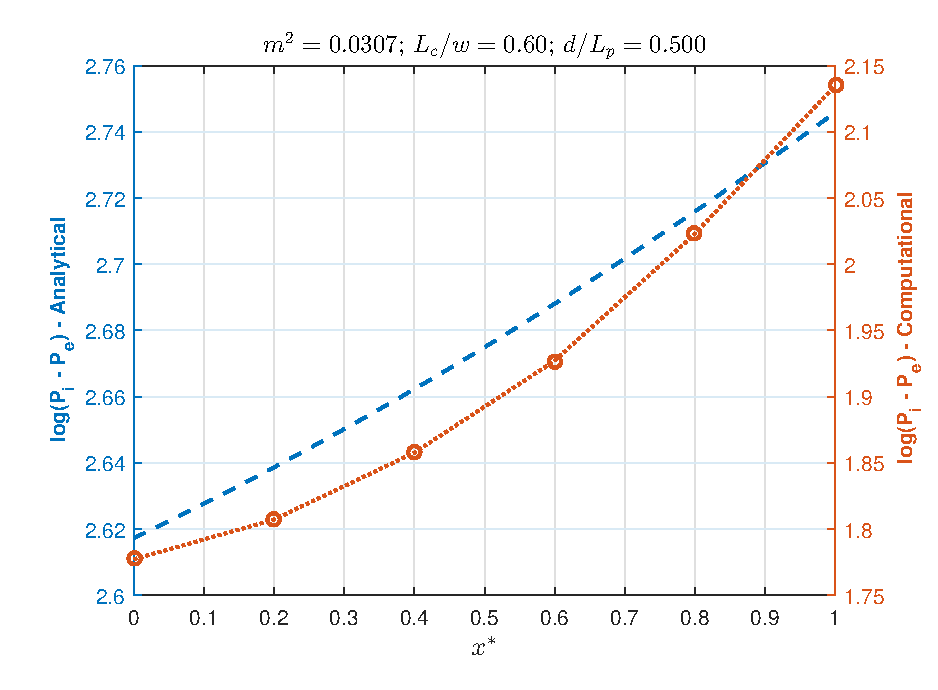
\includegraphics[height=0.55\linewidth,width=0.90\linewidth]{pres_c.eps}
   \caption{}
   \label{pres_c} 
\end{subfigure}
%
\caption{LOCAL PRESSURE DROPS}
\vspace{-3em}
\end{figure}
%
%
\subsection{Validation for Existence of Optimal Geometry}\label{optgeo}
We theoretically postulated the existence of an optimal channel size ratio ($d/L_p$) and a maximal heat transfer density ($q'''_{max}$) in section \ref{existence_dopt}. In this section, we numerically validate the existence of such an optimal configuration. 
%
\begin{figure}
\centering
   \begin{subfigure}[b]{0.55\textwidth}
   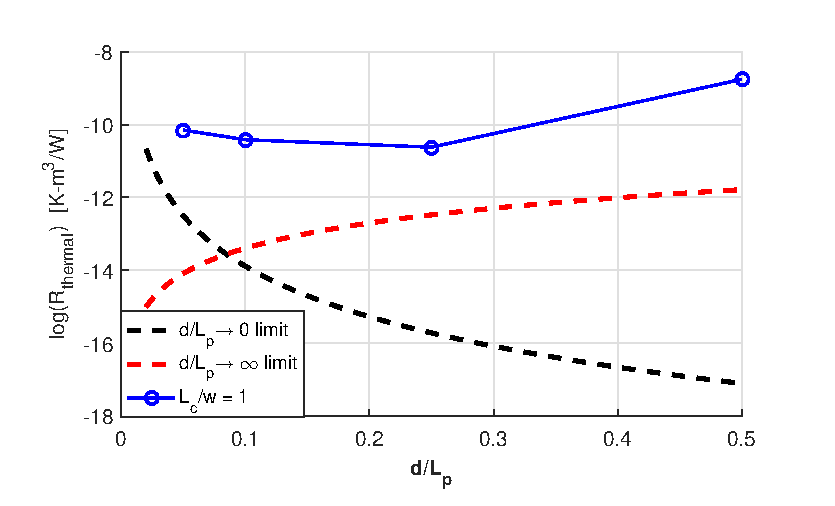
\includegraphics[width=0.85\linewidth]{Rmin_a.eps}
   \caption{}
   \label{Rmin_a} 
\end{subfigure}
%
   \begin{subfigure}[b]{0.55\textwidth}
   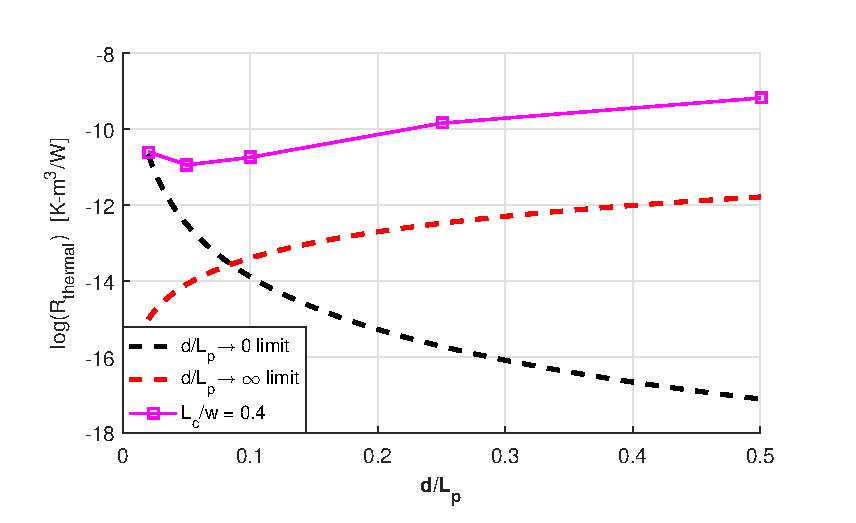
\includegraphics[width=0.85\linewidth]{Rmin_b.eps}
   \caption{}
   \label{Rmin_b} 
\end{subfigure}
%
%
   \begin{subfigure}[b]{0.55\textwidth}
   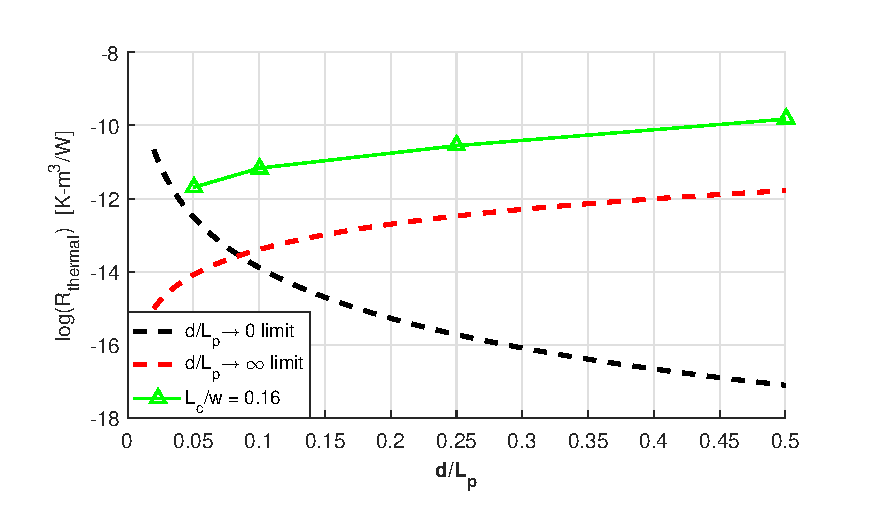
\includegraphics[width=0.85\linewidth]{Rmin_c.eps}
   \caption{}
   \label{Rmin_c} 
\end{subfigure}
%
\caption{EXISTENCE OF OPTIMAL GEOMETRY}
\vspace{-3em}
\end{figure}
%
%
The optimal channel size has been investigated for a number of different configurations by varying the diameter $ d $ (holding length of pore constant) and studying the variation of the heat transfer rate for different conduit lengths $L_C$ (holding width $w$ constant). Looking at the maximal $ q''' $ is equivalent to looking at the minimum thermal resistance $ R_{thermal} $ (K-m$^3$/W) where $ R_{thermal}=(T_w-T_{\infty})/q''' $. For a fixed pressure drop of 50 Pa, inlet velocity of 1 m/s, $w=0.025$m, $L_p=0.01$m, Figs. (\ref{Rmin_a}) and (\ref{Rmin_b}) show the existence of minimum $R_{thermal}$. The dotted curves in these figures are for the two asymptotes of eqs. (\ref{d0}) \& (\ref{dinf}). It is clear that with decreasing values of $L_C/w$, the minima shifts towards smaller and smaller values of $d/L_p$. It is because of this reason that the minima is not discernible in Fig. (\ref{Rmin_c}). All these CFD predictions for the optimal configuration that correspond to minimum $R_{thermal}$ are well within the vicinity of the optimal predicted through asymptotic analysis, thus demonstrating the feasibility of the method.  Although the model has somewhat under-predicted the value of $R_{thermal}$, the qualitative variations are very close to what one would expect.
%
\subsection{Optimal Channel Topology}\label{choiceofdesign}
\subsubsection*{Flow Distribution \& Need for Uniformity:} The heat transfer has to be optimised on two fronts. The macroscopic scale optimisation commands that the flow distribute evenly along the length of the inlet conduit; which is to say that the flow must, in the ideal case, divide itself uniformly as it leaks out of the inlet conduit into the exit conduit via the laterally stacked pores. The system, if not designed for the optimal case, will see the fluid entering the inlet conduit and taking the least resistance path which is the open conduit itself. In such a case, most of the fluid transitions to the exit conduit via a few pores located at the opposite end of the inlet conduit ($x \rightarrow 1$), while very little fluid passes through the pores located upstream close to the inlet. As a result, most of the length of porous material located close to the inlet will remain untouched by the fluid. This in turn implies that the system's surface area exposed for heat transfer is effectively very small and thereby the system does not perform maximally. Hence there is a need for ensuring good uniformity of flow in the lengthwise direction through a suitable choice of geometric design parameters.
%
\subsubsection*{Choice of design:} As discussed above, due to flow mal-distribution, a large fraction of the fluid passes through pores that are located close to $x=1$. As a result, the fluid velocities in these pores are very high as compared to those in pores located close to $x=0$. We can thus define a metric whose magnitude on either side of 0 measures the degree of flow deviation from the ideally desired uniform flow distribution. This metric `$ s $' is defined as
%
\[s = \frac{\parbox{7em}{\center{Maximum pore fluid velocity}}\,-\,\parbox{10em}{\center{Pore fluid velocity if flow were uniform}}}{\text{Inlet fluid velocity}}\]
%
The above section \ref{optgeo} discussed the existence of optimal range of $d/L_p$ that results in small values of $R_{thermal}$. But this approach maximises heat transfer rate at a microscopic level, resulting from a smart choice for porosity. Nevertheless, this choice of optimal porosity does not guarantee macroscopic heat transfer optimisation which would require an appreciable degree of flow evenness or in other words, as small a value of `$s$' as possible. Therefore, to arrive at a choice of porosity that addresses both microscopic as well as macroscopic heat transfer optimisation, we must look at both the `$s$' metric and $R_{thermal}$ as functions of $d/L_p$ for a given configuration and then choose the optimal $d/L_p$ (or equivalently the porosity) such that $s\rightarrow 0 $ and  $R_{thermal}$ is as low as possible. The results presented next are for constant width of conduit ($w$) and variable length of conduit $L_C$.
%
Fig. (\ref{optgeo_a}) shows that the $0.2 \leq \text{optimal } d/L_p \leq 0.26$ as such a choice enables $s$ to go to 0 as well as ensures a small enough value of the thermal resistance. Similarly, Fig. (\ref{optgeo_b}) suggests that $0.02 \leq \text{optimal } d/L_p \leq 0.06$ for $L_C/w=0.4$. Fig. (\ref{optgeo_c}) indicates that  $\text{optimal }d/L_p \leq 0.05$ for $L_C/w=0.16$. As a rule of thumb based on the graphs discussed and more analogical results from other configurations (not presented here for the sake of avoiding repetition), one can safely conclude that the choice of the optimal topology ($d/L_p$ or porosity) must be made in the range where $R_{thermal}$ sees a minima and should then be further refined by a minimisation of $s$.
%%%%
%
\begin{figure}
\centering
   \begin{subfigure}[b]{0.55\textwidth}
   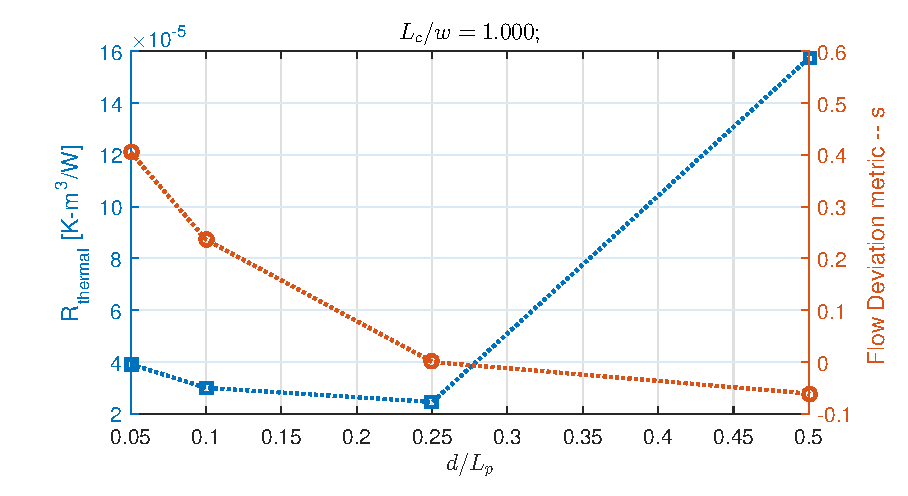
\includegraphics[width=0.85\linewidth]{optgeo_a.eps}
   \caption{}
   \label{optgeo_a} 
\end{subfigure}
%
   \begin{subfigure}[b]{0.55\textwidth}
   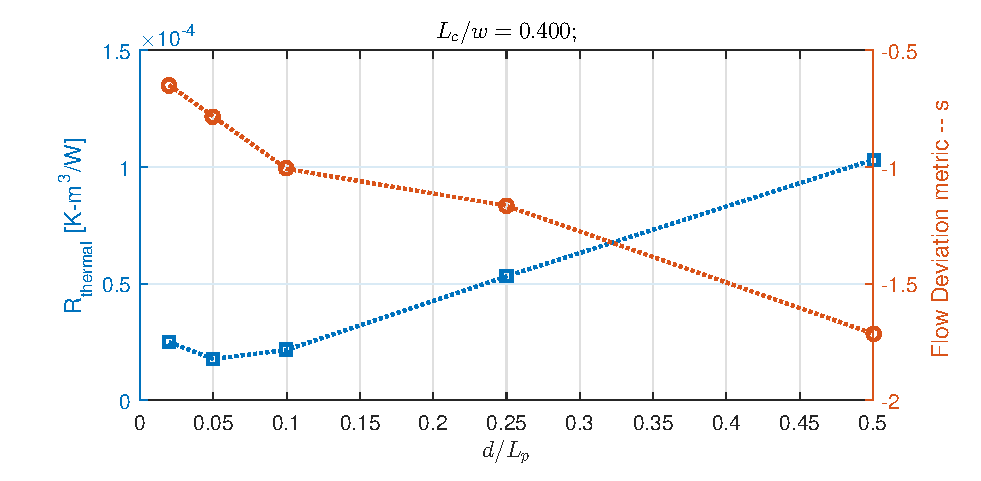
\includegraphics[width=0.85\linewidth]{optgeo_b.eps}
   \caption{}
   \label{optgeo_b} 
\end{subfigure}
%
%
   \begin{subfigure}[b]{0.55\textwidth}
   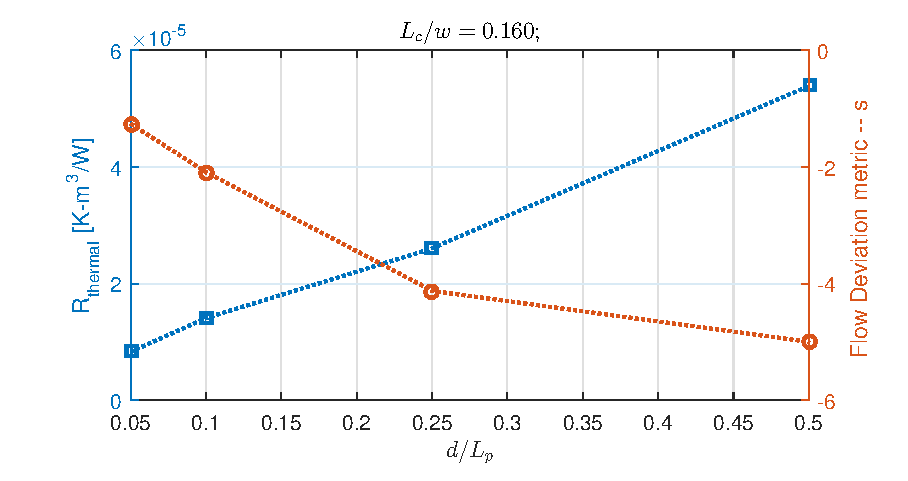
\includegraphics[width=0.85\linewidth]{optgeo_c.eps}
   \caption{}
   \label{optgeo_c} 
\end{subfigure}
%
\caption{CHOICE OF OPTIMAL CHANNEL TOPOLOGY}
\vspace{-3em}
\end{figure}
%
%
%%%%%%%%%%%%%%%%%%%%%%%%%%%%%%%%%%%%%%%%%%%%%%%%

\subsection{Optimal Number of Fins per Inch}\label{fpi}
So far we have considered a periodically repeating unit cell. But given a fixed length of heated substrate, what are the design rules for determination of the number of fins (or unit cells) that can be mounted over it? This question can be addressed by looking at the behaviour of $R_{thermal}$ as a function of variable width of the conduit $w$ holding the conduit length -- $L_C$ as constant. Over the range of $d/L_p$ investigated for variable $w$ configurations, the values of $R_{thermal}$ are seen to be monotonically increasing. More importantly, it is found that for a given porosity (or $d/L_p$), design configurations with smaller $w/L_C$ perform better in terms of offering lower thermal resistance -- $R_{thermal}$. These observations made from Fig. (\ref{fpi:fig}), along with discussion of section \ref{choiceofdesign} are instinctive and reveal the importance of selecting appropriate $w/L_C$ and $d/L_p$ for the design configuration. 
%
\begin{figure}[ht]
\centerline{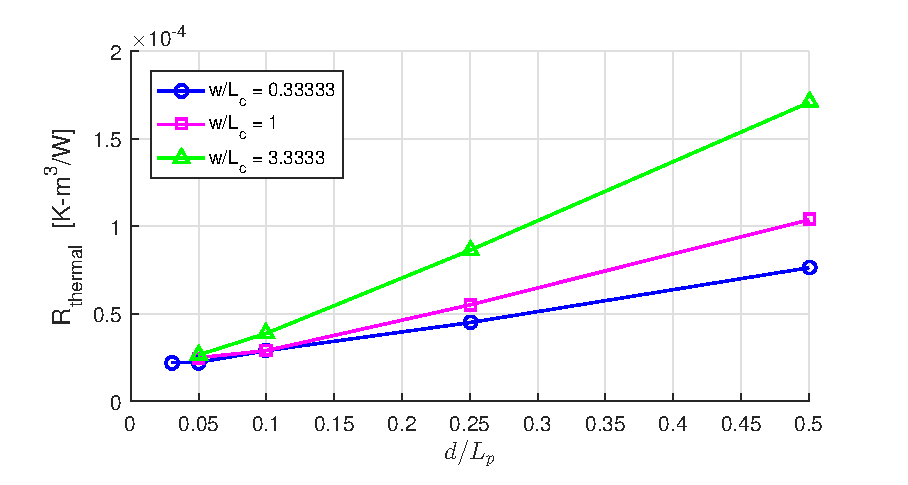
\includegraphics[width=1.1\linewidth]{fpi.eps}}
\vspace{-0.5em}
\caption{OPTIMAL FINS PER INCH (FPI)}
\vspace{-3em}
\label{fpi:fig}
\end{figure}

%%%%%%%%%%%%%
%%%%%%%%%%%%%%%%%%%%%%%%%%%%%%%%%%%%%%%%%%%%%%%%

\bibliographystyle{ihmtc}
\bibliography{ihmtc}

\end{document}
